\hypertarget{phonefirewall__administration_8c}{
\section{phonefirewall\_\-administration.c File Reference}
\label{phonefirewall__administration_8c}\index{phonefirewall\_\-administration.c@{phonefirewall\_\-administration.c}}
}
{\tt \#include $<$stdio.h$>$}\par
{\tt \#include $<$stdlib.h$>$}\par
{\tt \#include $<$errno.h$>$}\par
{\tt \#include $<$string.h$>$}\par
{\tt \#include \char`\"{}libphonefirewall.h\char`\"{}}\par


Include dependency graph for phonefirewall\_\-administration.c:\nopagebreak
\begin{figure}[H]
\begin{center}
\leavevmode
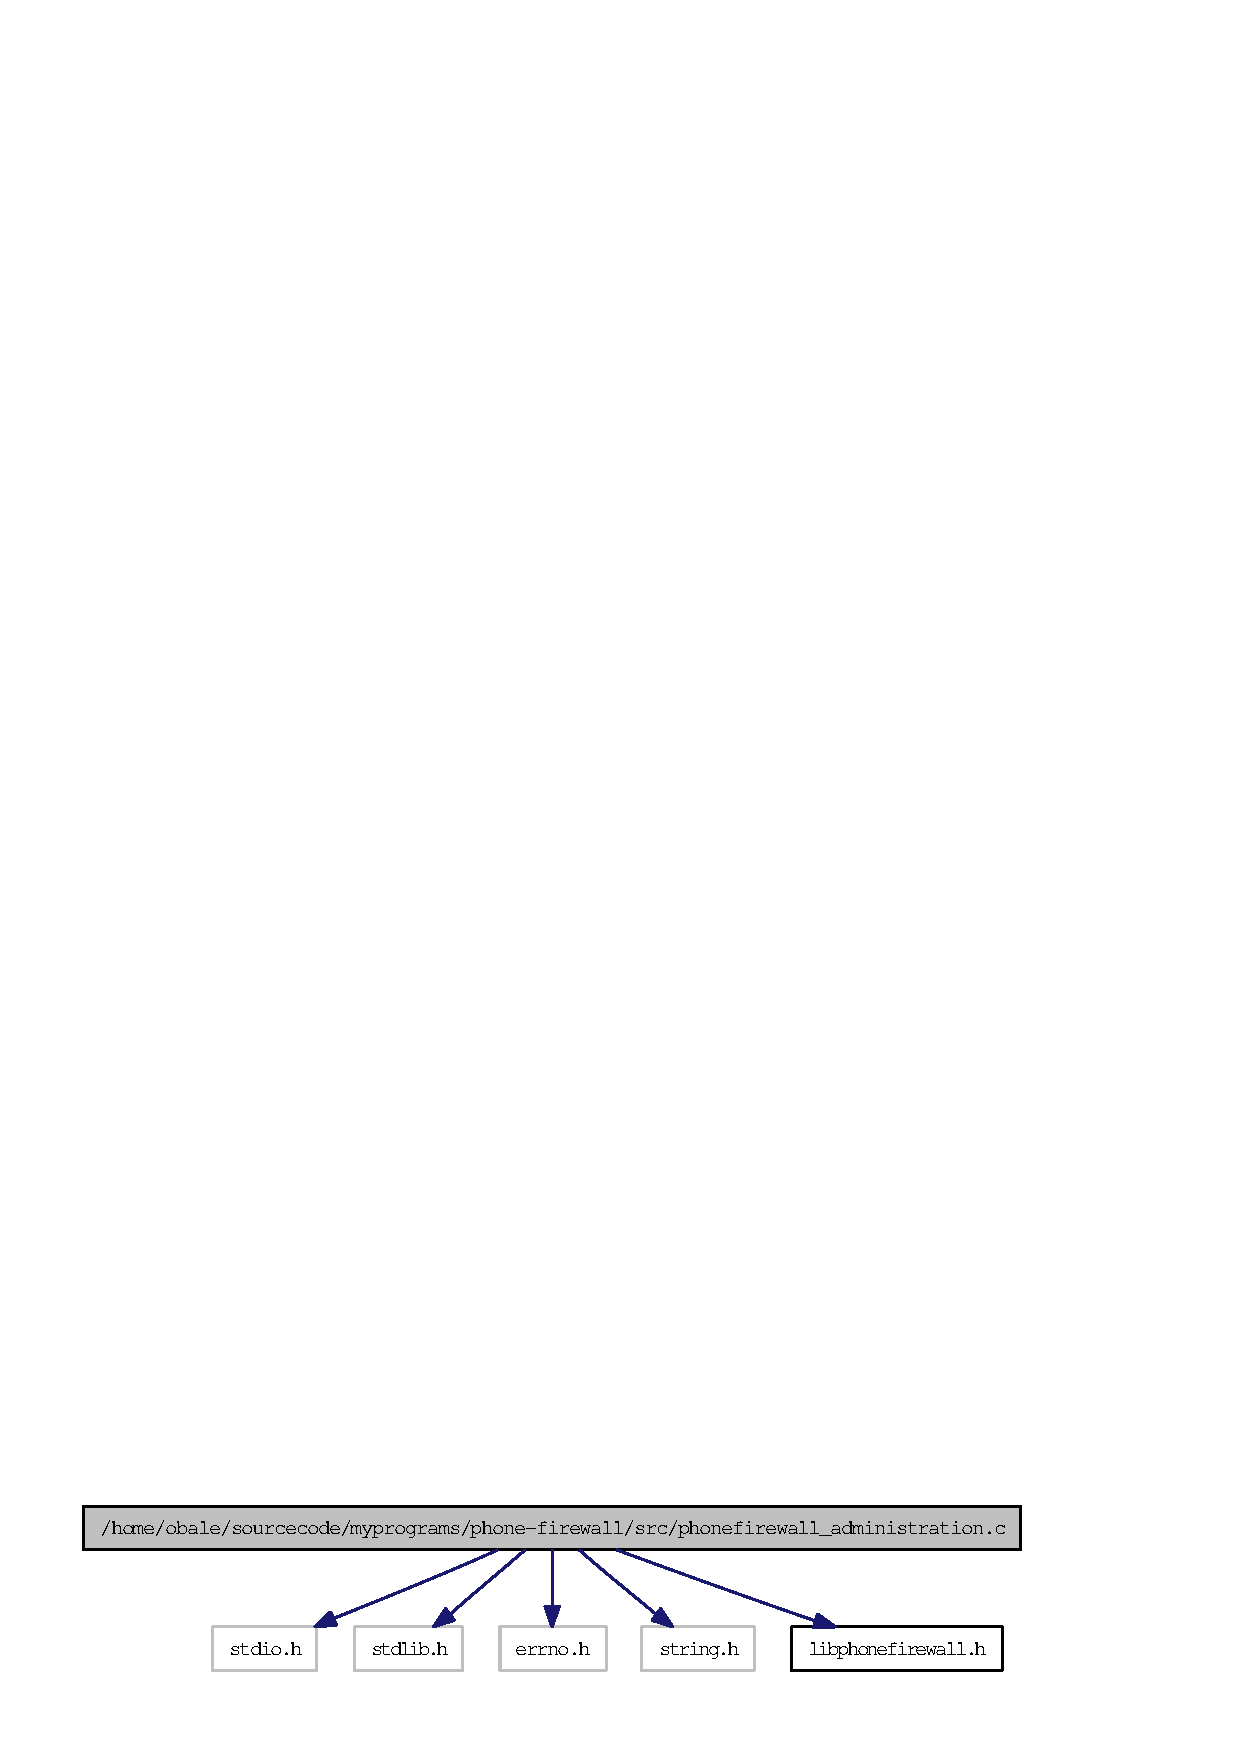
\includegraphics[width=211pt]{phonefirewall__administration_8c__incl}
\end{center}
\end{figure}
\subsection*{Typedefs}
\begin{CompactItemize}
\item 
typedef struct \hyperlink{structBlacklist}{Blacklist} \hyperlink{phonefirewall__administration_8c_423de6f8f476af2cac860172184b28f5}{blacklist\_\-t}
\item 
typedef struct \hyperlink{structWhitelist}{Whitelist} \hyperlink{phonefirewall__administration_8c_958e5a9da3b1faa340643f9f9e784fd5}{whitelist\_\-t}
\end{CompactItemize}
\subsection*{Functions}
\begin{CompactItemize}
\item 
\hyperlink{structBlacklist}{blacklist\_\-t} $\ast$ \hyperlink{phonefirewall__administration_8c_12ea11411729dc427517642a601f33dc}{add\_\-to\_\-blacklist} (\hyperlink{structBlacklist}{blacklist\_\-t} $\ast$node, long long int number, char $\ast$name, char $\ast$reason, int priority)
\item 
\hyperlink{structWhitelist}{whitelist\_\-t} $\ast$ \hyperlink{phonefirewall__administration_8c_7576c66d6eb51574047a4792cb88ee15}{add\_\-to\_\-whitelist} (\hyperlink{structWhitelist}{whitelist\_\-t} $\ast$node, long long int number, char $\ast$name, char $\ast$reason, int priority)
\item 
int \hyperlink{phonefirewall__administration_8c_23f18831c9677c1a3b7f8cb6b20f3e02}{add\_\-blacklist\_\-entry} (long long int number, char $\ast$name, char $\ast$reason, int priority)
\item 
int \hyperlink{phonefirewall__administration_8c_c1875490cf592d507798a292f8a772e9}{rm\_\-blacklist\_\-entry} (long long int number)
\item 
int \hyperlink{phonefirewall__administration_8c_2f8998691bfe087c701006c9efd2a6cd}{add\_\-whitelist\_\-entry} (long long int number, char $\ast$name, char $\ast$reason, int priority)
\item 
int \hyperlink{phonefirewall__administration_8c_c3a77117dbcade02ab233836e559814a}{rm\_\-whitelist\_\-entry} (long long int number)
\end{CompactItemize}


\subsection{Typedef Documentation}
\hypertarget{phonefirewall__administration_8c_423de6f8f476af2cac860172184b28f5}{
\index{phonefirewall\_\-administration.c@{phonefirewall\_\-administration.c}!blacklist\_\-t@{blacklist\_\-t}}
\index{blacklist\_\-t@{blacklist\_\-t}!phonefirewall_administration.c@{phonefirewall\_\-administration.c}}
\subsubsection{\setlength{\rightskip}{0pt plus 5cm}typedef struct {\bf Blacklist} {\bf blacklist\_\-t}}}
\label{phonefirewall__administration_8c_423de6f8f476af2cac860172184b28f5}




Definition at line 26 of file phonefirewall\_\-administration.c.\hypertarget{phonefirewall__administration_8c_958e5a9da3b1faa340643f9f9e784fd5}{
\index{phonefirewall\_\-administration.c@{phonefirewall\_\-administration.c}!whitelist\_\-t@{whitelist\_\-t}}
\index{whitelist\_\-t@{whitelist\_\-t}!phonefirewall_administration.c@{phonefirewall\_\-administration.c}}
\subsubsection{\setlength{\rightskip}{0pt plus 5cm}typedef struct {\bf Whitelist} {\bf whitelist\_\-t}}}
\label{phonefirewall__administration_8c_958e5a9da3b1faa340643f9f9e784fd5}




Definition at line 27 of file phonefirewall\_\-administration.c.

\subsection{Function Documentation}
\hypertarget{phonefirewall__administration_8c_23f18831c9677c1a3b7f8cb6b20f3e02}{
\index{phonefirewall\_\-administration.c@{phonefirewall\_\-administration.c}!add\_\-blacklist\_\-entry@{add\_\-blacklist\_\-entry}}
\index{add\_\-blacklist\_\-entry@{add\_\-blacklist\_\-entry}!phonefirewall_administration.c@{phonefirewall\_\-administration.c}}
\subsubsection{\setlength{\rightskip}{0pt plus 5cm}int add\_\-blacklist\_\-entry (long long int {\em number}, char $\ast$ {\em name}, char $\ast$ {\em reason}, int {\em priority})}}
\label{phonefirewall__administration_8c_23f18831c9677c1a3b7f8cb6b20f3e02}


Add a number to the blacklist. The number will be blocked after that.

\begin{Desc}
\item[Parameters:]
\begin{description}
\item[{\em number}]The telephone number of the person. \item[{\em name}]The name of the person. \item[{\em reason}]Why you have blocked this person. \item[{\em priority}]Has no affect at the moment. Later one it will be possible to give each number priority. So you have more control when a number will be blocked/accepted.\end{description}
\end{Desc}
\begin{Desc}
\item[Returns:]If all goes well 0 (zero) otherwise an errno code. \end{Desc}


Definition at line 66 of file phonefirewall\_\-administration.c.

References add\_\-to\_\-blacklist().

Here is the call graph for this function:\nopagebreak
\begin{figure}[H]
\begin{center}
\leavevmode
\includegraphics[width=144pt]{phonefirewall__administration_8c_23f18831c9677c1a3b7f8cb6b20f3e02_cgraph}
\end{center}
\end{figure}
\hypertarget{phonefirewall__administration_8c_12ea11411729dc427517642a601f33dc}{
\index{phonefirewall\_\-administration.c@{phonefirewall\_\-administration.c}!add\_\-to\_\-blacklist@{add\_\-to\_\-blacklist}}
\index{add\_\-to\_\-blacklist@{add\_\-to\_\-blacklist}!phonefirewall_administration.c@{phonefirewall\_\-administration.c}}
\subsubsection{\setlength{\rightskip}{0pt plus 5cm}{\bf blacklist\_\-t}$\ast$ add\_\-to\_\-blacklist ({\bf blacklist\_\-t} $\ast$ {\em node}, long long int {\em number}, char $\ast$ {\em name}, char $\ast$ {\em reason}, int {\em priority})}}
\label{phonefirewall__administration_8c_12ea11411729dc427517642a601f33dc}




Definition at line 29 of file phonefirewall\_\-administration.c.

References Blacklist::left, Blacklist::name, Blacklist::number, Blacklist::priority, Blacklist::reason, and Blacklist::right.

Referenced by add\_\-blacklist\_\-entry().\hypertarget{phonefirewall__administration_8c_7576c66d6eb51574047a4792cb88ee15}{
\index{phonefirewall\_\-administration.c@{phonefirewall\_\-administration.c}!add\_\-to\_\-whitelist@{add\_\-to\_\-whitelist}}
\index{add\_\-to\_\-whitelist@{add\_\-to\_\-whitelist}!phonefirewall_administration.c@{phonefirewall\_\-administration.c}}
\subsubsection{\setlength{\rightskip}{0pt plus 5cm}{\bf whitelist\_\-t}$\ast$ add\_\-to\_\-whitelist ({\bf whitelist\_\-t} $\ast$ {\em node}, long long int {\em number}, char $\ast$ {\em name}, char $\ast$ {\em reason}, int {\em priority})}}
\label{phonefirewall__administration_8c_7576c66d6eb51574047a4792cb88ee15}




Definition at line 48 of file phonefirewall\_\-administration.c.

References Whitelist::left, Whitelist::name, Whitelist::number, Whitelist::priority, Whitelist::reason, and Whitelist::right.\hypertarget{phonefirewall__administration_8c_2f8998691bfe087c701006c9efd2a6cd}{
\index{phonefirewall\_\-administration.c@{phonefirewall\_\-administration.c}!add\_\-whitelist\_\-entry@{add\_\-whitelist\_\-entry}}
\index{add\_\-whitelist\_\-entry@{add\_\-whitelist\_\-entry}!phonefirewall_administration.c@{phonefirewall\_\-administration.c}}
\subsubsection{\setlength{\rightskip}{0pt plus 5cm}int add\_\-whitelist\_\-entry (long long int {\em number}, char $\ast$ {\em name}, char $\ast$ {\em reason}, int {\em priority})}}
\label{phonefirewall__administration_8c_2f8998691bfe087c701006c9efd2a6cd}


Add a number to the whitelist. The number will be accepted after that.

\begin{Desc}
\item[Parameters:]
\begin{description}
\item[{\em number}]The telephone number of the person. \item[{\em name}]The name of the person. \item[{\em reason}]Why you have blocked this person. \item[{\em priority}]Has no affect at the moment. Later one it will be possible to give each number priority. So you have more control when a number will be blocked/accepted.\end{description}
\end{Desc}
\begin{Desc}
\item[Returns:]If all goes well 0 (zero) otherwise an errno code. \end{Desc}


Definition at line 78 of file phonefirewall\_\-administration.c.\hypertarget{phonefirewall__administration_8c_c1875490cf592d507798a292f8a772e9}{
\index{phonefirewall\_\-administration.c@{phonefirewall\_\-administration.c}!rm\_\-blacklist\_\-entry@{rm\_\-blacklist\_\-entry}}
\index{rm\_\-blacklist\_\-entry@{rm\_\-blacklist\_\-entry}!phonefirewall_administration.c@{phonefirewall\_\-administration.c}}
\subsubsection{\setlength{\rightskip}{0pt plus 5cm}int rm\_\-blacklist\_\-entry (long long int {\em number})}}
\label{phonefirewall__administration_8c_c1875490cf592d507798a292f8a772e9}


Removes a blocked number from the blacklist. 

Definition at line 74 of file phonefirewall\_\-administration.c.\hypertarget{phonefirewall__administration_8c_c3a77117dbcade02ab233836e559814a}{
\index{phonefirewall\_\-administration.c@{phonefirewall\_\-administration.c}!rm\_\-whitelist\_\-entry@{rm\_\-whitelist\_\-entry}}
\index{rm\_\-whitelist\_\-entry@{rm\_\-whitelist\_\-entry}!phonefirewall_administration.c@{phonefirewall\_\-administration.c}}
\subsubsection{\setlength{\rightskip}{0pt plus 5cm}int rm\_\-whitelist\_\-entry (long long int {\em number})}}
\label{phonefirewall__administration_8c_c3a77117dbcade02ab233836e559814a}


Removes a accepted number from the whitelist. 

Definition at line 82 of file phonefirewall\_\-administration.c.